%% Markowitz-Portfolio.txt
%% Mac Radigan
%
%% Markowitz Portfolio Example Documentation

\documentclass{article}[11pt]
\usepackage[]{graphics}
\usepackage{titlesec}

\usepackage[framed,numbered,autolinebreaks,useliterate]{mcode}
\usepackage{setspace}
\usepackage[left=1in,top=1in,right=1in,bottom=1in,nohead]{geometry}
\usepackage{graphicx,amssymb,amstext,amsmath,amsthm,caption,mathtools}
\usepackage{algorithm}
\usepackage{algorithmic}
\usepackage{amsfonts}
\usepackage{amssymb}
\bibliographystyle{IEEEtran}
\usepackage{csvtools}
\usepackage{pdftexcmds}
\usepackage{minted}
\usepackage{fancyvrb}
\usepackage{float}
\usepackage{epstopdf}
%\titleformat{\section}[block]{\Large\bfseries\filcenter}{}{}{}
%\newcommand\Quote[1]{\lq\textsl{#1}\rq}
%\newcommand\fr[2]{{\textstyle\frac{#1}{#2}}}
%\newcommand{\ssection}[1]{\section[#1]{\centering\normalfont\scshape #1}}
%\newcommand{\ssubsection}[1]{\subsection[#1]{\raggedright\normalfont\itshape #1}}

\begin{document}

\title{Markowitz Portfolio Example}
\author{Mac Radigan}
\date{} % comment this out if you would like to include the date
\doublespacing

\maketitle

%\nocite{*}

%\begin{abstract}
%\end{abstract}

%\tableofcontents
%\listoffigures

\subsection{Introduction}
Markowitz portfolio theory is used in investment management 
as a tool for diversifying away risk through portfolio balancing.
Given a set of investment assets, it finds the most efficient  
allocation (portfolio weights).  Here, efficiency is defined  
as minimizing the expected variance.  Markowitz portfolios
may be subject to specified constraints, such as a specific 
return on investment (expected price), non-negativity 
constraints (restricting short selling), and may include 
risk-free assets or market indexes \cite{WikiMPT}.
\newline

This example will select a minimum variance portfolio,
constrained to a specified expected rate of return.
All results will be annualized as commonly reported to
investors.
\newline

\subsection{Implementation}

This optmization problem may be expressed as minimizing the portfolio variance, 
subject to the constraint that the individual allocation weights of the stocks add to unity,
and the expected return is equal to the specified target.
\newline

\begin{equation*}
\begin{aligned}
& \underset{w}{\text{minimize}}
& & \mathbf{\sigma}_{p,w}^2 = \mathbf{w}^T \mathbf{\Sigma} \mathbf{w} \\
& \text{subject to}
& & \mu_{opt} = \mathbf{w}^T \mathbf{\mu} \\
&
& & \mathbf{w}^T \mathbf{\underline{1}} = 1
\end{aligned}
\label{eq:optimization_problem}
\end{equation*}

Where
\begin{subequations}
%\tag{Notation}
\begin{align}
\begin{array}{cl}
\mathbf{\sigma}_{p,w}^2      & \mbox{portfolio variance of weighted assets} \\
\mathbf{w}         & \mbox{individual asset weights}  \\
\mathbf{\Sigma}    & \mbox{covariance matrix} \\
\mathbf{\mu}       & \mbox{individual asset returns} \\
\mathbf{\mu}_{opt} & \mbox{target portfolio return} \\
\end{array}
\end{align}
\label{eq:notation}
\end{subequations}

Forming the Lagrangian function for the constrained minimization, we have

\begin{equation}
L(w,\lambda_1,\lambda_2) = \mathbf{w}^T \mathbf{\Sigma} \mathbf{w} + \lambda_1 (\mathbf{w}^T \mathbf{\mu} - \mu_{opt})
\label{eq:lagrangian}
\end{equation}

So the first order conditions are

\begin{equation}
2 \partial L(w,\lambda_1,\lambda_2) = 2 \mathbf{\Sigma} \mathbf{w} + \lambda_1 \mathbf{\mu} + \lambda_2 \mathbf{\underline{1}} = \mathbf{\underline{0}}
\label{eq:foc1}
\end{equation}

\begin{equation}
\frac{2 \partial L(w,\lambda_1,\lambda_2)}{\partial \lambda_1} = \mathbf{w}^T \mathbf{\mu} - \mu_{opt} = 0
\label{eq:foc2}
\end{equation}

\begin{equation}
\frac{2 \partial L(w,\lambda_1,\lambda_2)}{\partial \lambda_2} = \mathbf{w}^T \mathbf{\underline{1}} - 1 = 0
\label{eq:foc3}
\end{equation}

Expressed in matrix form

\begin{equation}
\mathbf{A}\mathbf{x} =
\left[ \begin{array}{ccc}
2 \mathbf{\Sigma}         & \mathbf{\mu} & \mathbf{\underline{1}} \\
\mathbf{\mu}^T            & 0            & 0                      \\
\mathbf{\underline{1}}^T  & 0            & 0                      \\
\end{array} \right]
=
\left[ \begin{array}{c}
\mathbf{w} \\
\lambda_1  \\
\lambda_2  \\
\end{array} \right]
\left[ \begin{array}{c}
\mathbf{\underline{0}}^T \\
\mu_{opt}  \\
1  \\
\end{array} \right]
= \mathbf{b}
\label{eq:lineq_expand}
\end{equation}

This may be solved for $\mathbf{b}$, where the first $n-2$ elements of $\mathbf{b}$ are the portfolio weights ($\mathbf{w}_{n} = \mathbf{b}_{n}$).

\begin{equation}
\mathbf{b} = \mathbf{A}^{-1} \mathbf{x}
\label{eq:lineq_mat}
\end{equation}

\bibliography{IEEEabrv,bibliography}

%% Appendix-Portfolio.tex
%% Mac Radigan
%
%% Portfolio summary results from from Markowitz-C++ Example

\section{Appendix A: The Example Portfolio}
\label{sec:appendix_a}

\subsection{Portfolio \#1: AAPL, JPM, LMT, XOM}

\newline

\begin{table}[!ht]
\begin{center}
\begin{tabular}{ l l l l }
\toprule
\multicolumn{5}{ c }{ \textbf{Portfolio \#1 (AAPL, JPM, LMT, XOM)} } \\
\hline
\textbf{Symbol} & \textbf{Weight} & \textbf{ROI} & \textbf{Volatilty} \\ \hline
AAPL   & 0.08 & 11.4\% & 28.8\% \\
JPM    & 0.12 & 31.6\% & 19.1\% \\
LMT    & 0.39 & 55.8\% & 16.3\% \\
XOM    & 0.40 & 08.2\% & 13.0\% \\ 
\hline
portfolio & &  25.0\% & 11.76\% \\ 
\hline
\bottomrule
\end{tabular}
\caption{Portfolio \#1}
\end{center}
\end{table}

\newline

\begin{figure}[H]
\begin{center}
\resizebox{7in}{!}{\includegraphics{results/portfolios/AAPL_JPM_LMT_XOM/Portfolio.eps}}
%\includegraphics{results/AAPL_JPM_LMT_XOM/Portfolio.eps}
\end{center}
\caption{Portfolio Performance}
\label{fig:portfolio_aapl_jnj_lmt_xom}
\end{figure}


%% *EOF*


%% Appendix-Charts.tex
%% Mac Radigan
%
%% Stock chart results from Markowitz-C++ Example

\section{Appendix B: Historical Data}
\label{sec:appendix_b}

\subsection{AAPL Stock Chart}
\begin{figure}[H]
\begin{center}
%\resizebox{7in}{!}{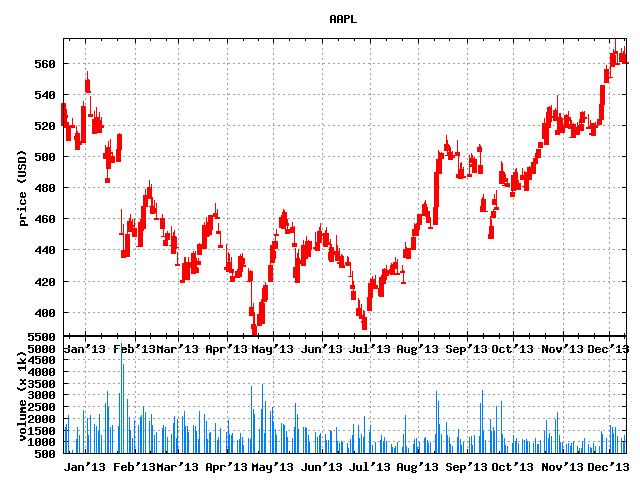
\includegraphics{./results/portfolios/AAPL_JPM_LMT_XOM/AAPL.eps}}
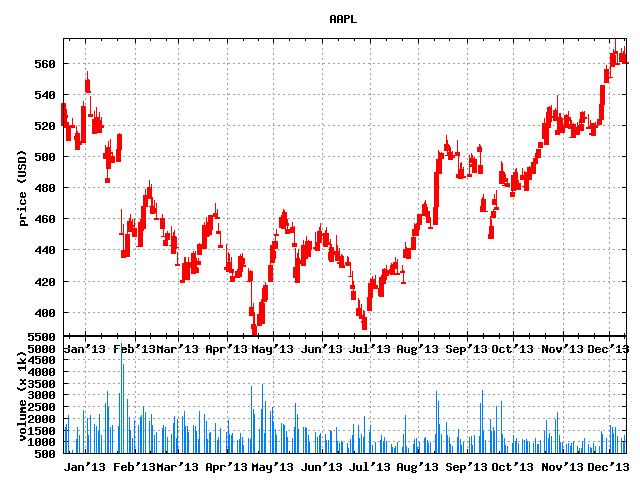
\includegraphics{./results/portfolios/AAPL_JPM_LMT_XOM/AAPL.eps}
\end{center}
\caption{AAPL}
\label{fig:history_aapl}
\end{figure}

\subsection{JPM Stock Chart}
\begin{figure}[H]
\begin{center}
%\resizebox{7in}{!}{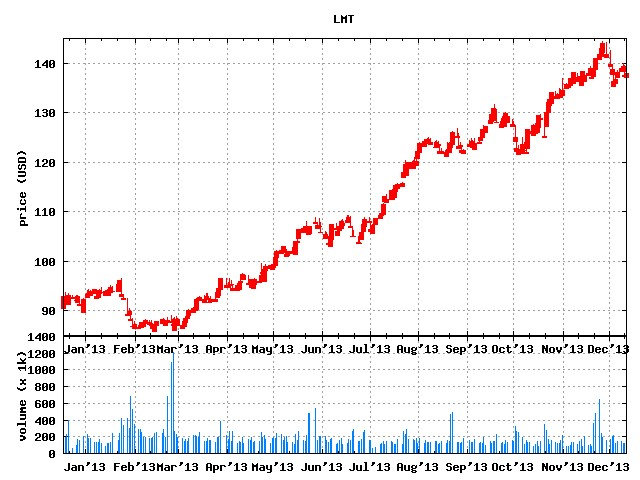
\includegraphics{./results/portfolios/AAPL_JPM_LMT_XOM/LMT.eps}}
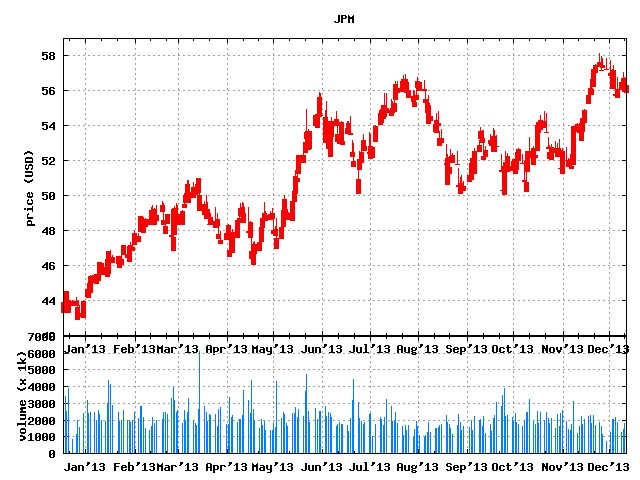
\includegraphics{./results/portfolios/AAPL_JPM_LMT_XOM/JPM.eps}
\end{center}
\caption{JPM}
\label{fig:history_jnj}
\end{figure}

\subsection{LMT Stock Chart}
\begin{figure}[H]
\begin{center}
%\resizebox{7in}{!}{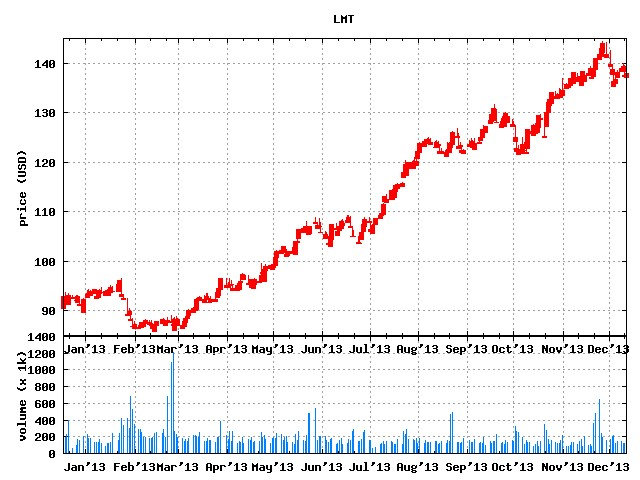
\includegraphics{./results/portfolios/AAPL_JPM_LMT_XOM/LMT.eps}}
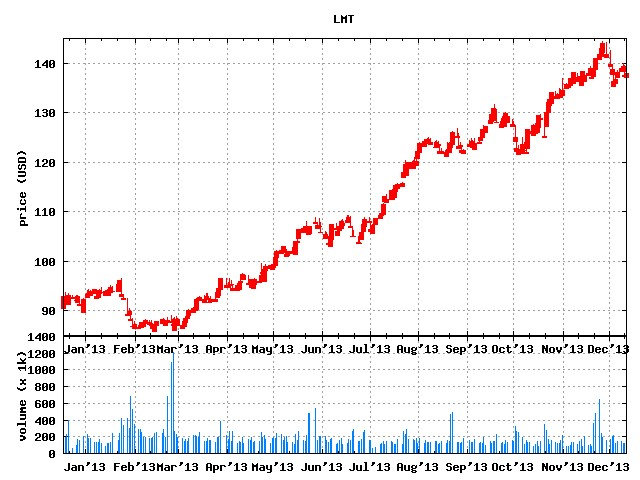
\includegraphics{./results/portfolios/AAPL_JPM_LMT_XOM/LMT.eps}
\end{center}
\caption{LMT}
\label{fig:history_lmt}
\end{figure}

\subsection{XOM Stock Chart}
\begin{figure}[H]
\begin{center}
%\resizebox{7in}{!}{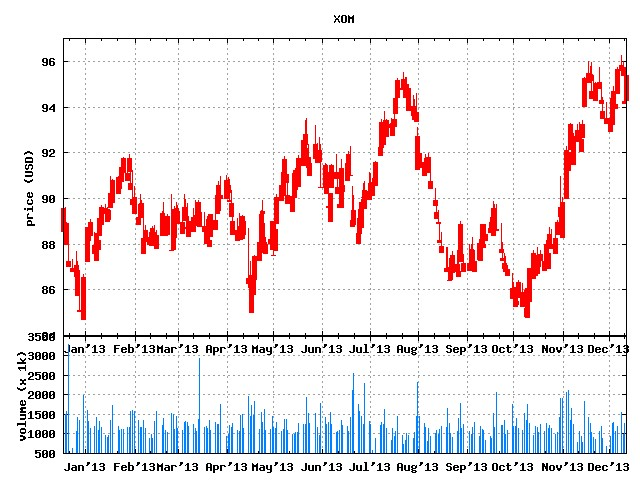
\includegraphics{./results/portfolios/AAPL_JPM_LMT_XOM/XOM.eps}}
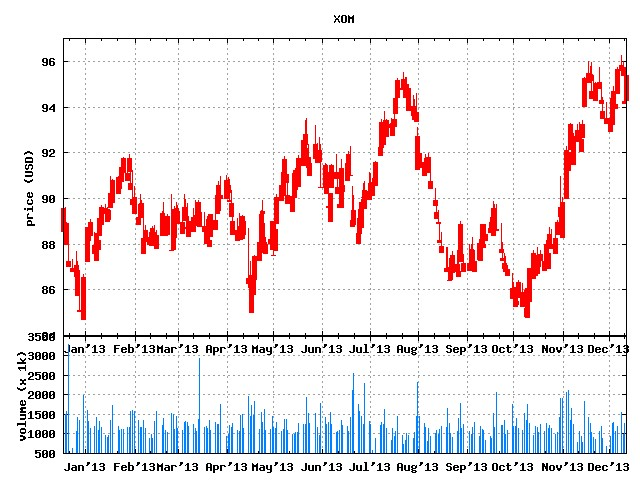
\includegraphics{./results/portfolios/AAPL_JPM_LMT_XOM/XOM.eps}
\end{center}
\caption{XOM}
\label{fig:history_xom}
\end{figure}

%% *EOF*


%% Appendix-SourceCode.tex
%% Mac Radigan
%
%% Octave source code listing

\section{Appendix C: Octave Source Code}
\label{sec:appendix_c}

\subsection{Appendix C.1: script example (main entry point)}
\label{sec:markowitzDemo_m}
\lstinputlisting{../octave/markowitzDemo.m}

\subsection{Appendix C.2: Markowitz Portfolio optimization function}
\label{sec:markowitzPortfolio_m}
\lstinputlisting{../octave/markowitzPortfolio.m}

\subsection{Appendix C.3: Stock Data Reader}
\label{sec:getStockData_m}
\lstinputlisting{../octave/getStockData.m}

%% *EOF*


\end{document}

%% %EOF*
